\documentclass[adobefonts, nocap]{ctexart}
\usepackage{amsmath}
\usepackage{amsfonts}
\usepackage{listings}
\usepackage{xcolor}
\usepackage{graphicx}
\usepackage{siunitx}
\usepackage{hyperref}
\hypersetup{
  colorlinks = true,
  linkcolor = blue,
  unicode = true
}
\lstset{
  language = C,
  basicstyle = \small\ttfamily,
  keywordstyle = \small\ttfamily\color{red},
  stringstyle = \color{gray},
  numbers = left,
  numberstyle = \tiny,
  numbersep = 5pt,
  frame = leftline,
  showstringspaces = false
}
\begin{document}
  \title{计算机系统结构第一次实验}
  \author{李雨田\hspace{1em}2010012193\hspace{1em}计14}
  \maketitle
  \tableofcontents
  \section{测量数据缓存的大小}
    \subsection{实验原理}
      基本思想是对一段大小的数据反复读取,并且逐次增加数据的大小.当数据的大小超过缓存的大小时,频繁读取会导致频繁
      替换缓存,使得吞吐量下降.所以只要测量吞吐量,观察发现突变的点,即可得到缓存的大小.

      但是最新的Intel处理器自带硬件预读取功能,即会根据程序执行的步长预测下一次访问,并且提前读取到内存里.如果
      按照顺序访问数组的方法,结果发现吞吐量一直不会下降,正是因为硬件预读取提前替换了缓存,没有影响到读取的效率.

      为了不让处理器预测出访问的步长,可以每次产生一个伪随机数作为下标访问.但是产生随机数会影响吞吐量的测试,并且
      调用外部函数时会导致内存访问,使得之前的缓存失效.所以只能仿照链表的实现方式,把下一次访问的地址放在这次访问
      的地址所对应的变量中.并且合理增大步长,加大替换缓存的次数.
    \subsection{实验结果和数据分析}
      运行程序,对1KB到2048KB之间大小都进行测试,并且得出吞吐量.吞吐量的单位是MB/s,但是因为使用\texttt{clock()}
      函数记时并不是很准确.不过最重要的是相对数值,所以并不影响测量缓存的大小.

      源代码为\texttt{cache-size.c},运行时通过命令行提供两个参数,分别为起始和结束测量的大小.然后程序会给出相应大小
      下的吞吐量.

      程序输出如图\ref{fig1}所示,结果如图\ref{fig2}所示.注意到横轴对应的是$2^{x}$KB.可以看出在32KB和256KB处有明显的吞吐量的突降,于是知道L1和L2数据缓存的大小分别为
      32KB和256KB.

      \begin{figure}[htbp]
        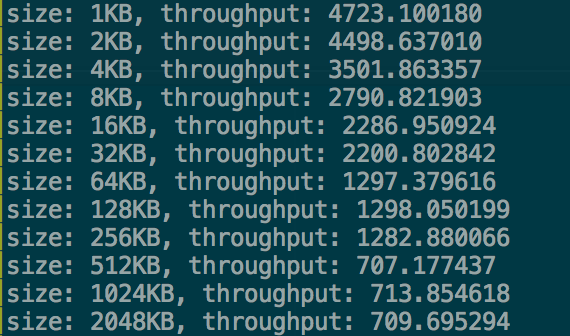
\includegraphics[width=12cm]{1.png}
        \caption{数据缓存大小程序输出}
        \label{fig1}
      \end{figure}

      \begin{figure}[htbp]
        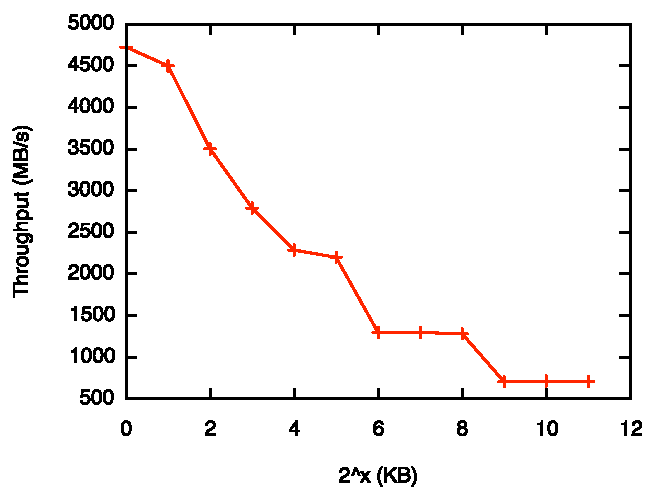
\includegraphics[width=12cm]{2.pdf}
        \caption{数据缓存大小数据}
        \label{fig2}
      \end{figure}
      \clearpage
  \section{测量数据缓存的块大小}
    \subsection{实验原理}
      同样是对内存进行顺序访问,但是读到块里的某一个字节时,整个块都会被缓存进来.所以如果按字节顺序访问,仅仅会在访问该块的第一个
      字节的时候对访问更低级存储,接下来在该块内的访问会更快.如果不每个字节都依次访问,加大访问的步长,可以预见当步长等于块大小的时候,
      每一次读取就会要访问更低级存储,将整个块都加载进来,这样的吞吐量是最低的.每次逐次加大步长的话,将会出现吞吐量先降后升.最低点对应的
      步长即是块大小.

      这里任然要注意到硬件预读取带来的影响,同样使用类似链表的数据结构.
    \subsection{实验结果和数据分析}
      程序源代码为\texttt{block-size.c}.运行程序,对步长从1到32进行测试.这里的步长是指\texttt{uint64\_t}的长度,即64B.

      得到程序输出如图\ref{fig3}

      \begin{figure}[htbp]
        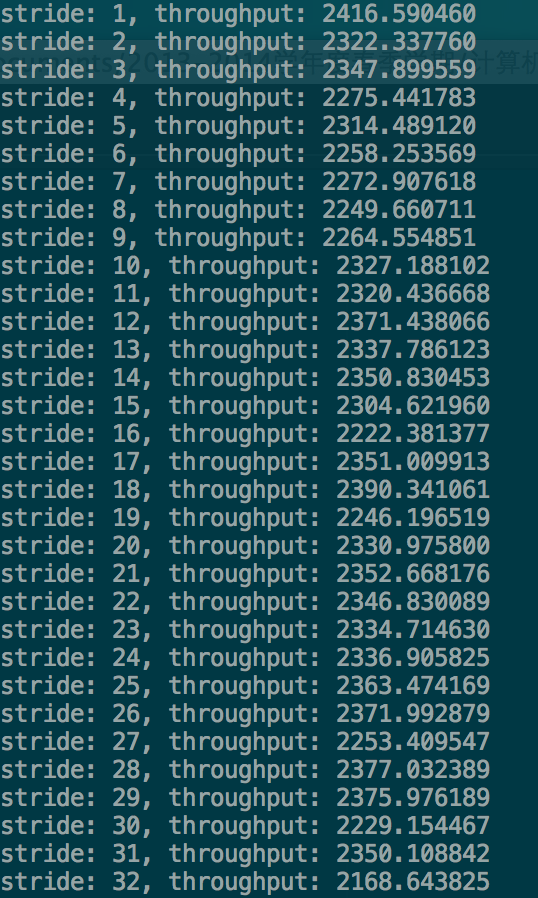
\includegraphics[width=12cm]{3.png}
        \caption{数据缓存块大小程序输出}
        \label{fig3}
      \end{figure}

      \begin{figure}[htbp]
        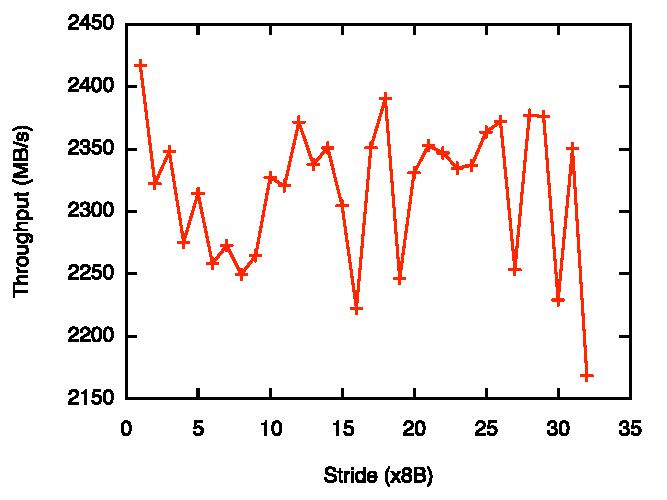
\includegraphics[width=12cm]{4.pdf}
        \caption{数据缓存块大小数据}
        \label{fig4}
      \end{figure}
      \clearpage
  \section{测量数据缓存的相连度}
    \subsection{实验原理}
      到现在已经知道块大小是64B,缓存的大小也已经测出来了.下面只要测出来一共有多少个组,就能知道每个组的大小和相连度了.

      已知块大小是64B,占了地址最低的6位.取一个掩码,用来分割地址前面的标签和后面的索引和偏移量部分.实际上可以取这个掩码加一的值,
      每次往地址上加这个值.如果掩码没有盖住索引和偏移量部分,那么往地址上加的时候会改变索引,会从一个组跳到另一个组.如果掩码正好盖住
      或者超过了索引和偏移量,那么往地址上递增的时候就只会改变标签,而任然还在同一个组内.

      所以通过依次左移掩码,当掩码正好盖住索引和偏移量的时候,所有读取的内容都属于同一个缓存组,缓存冲突频率最大,吞吐量最低.通过观察
      吞吐量下降到极值这个点,即可算出相连度.
    \subsection{实验结果和数据分析}
      程序源代码为\texttt{associativity.c}.依次左移掩码,得到程序输出如图\ref{fig5}.这里的\texttt{mask}实际上是掩码加一的值,
      即往地址上累加的值.

      数据如图\ref{fig6}.可以看出当掩码为12位的时候吞吐量最低,即地址的低12位是索引和偏移量.偏移量为6位,所以索引为6位,共有64组.一级缓存共有32KB,而块大小
      之前已经算出来是64B,计算得到一组里有8个块,即时8相连的.

      考虑到一级缓存和二级缓存有一定的一致性,猜测二级缓存也是8相连的.之前已经得到二级缓存共256KB,算得一共应有512组.对应的掩码有15位,
      可以看到如图\ref{fig6}当掩码为15位时,吞吐率的增长趋势得到抑制,验证猜测是正确的.

      对于图\ref{fig6}后面吞吐量开始上升,是因为程序采用固定读取量,测量时间得到吞吐量.当掩码变大时,实际上每一步跳跃距离变大,但数组大小不变,
      为了达到同样的读取量,只能多次重复读取.很可能即使是在同一组中,但因为不同的地址的数量太少,无法使这个组的缓存填满,更不用说替换缓存了,所以吞吐量
      会变高.要解决这个问题可以扩大数组的大小,但是实际上目前已经可以得到缓存的相连度,并没有这个必要.

      \begin{figure}[htbp]
        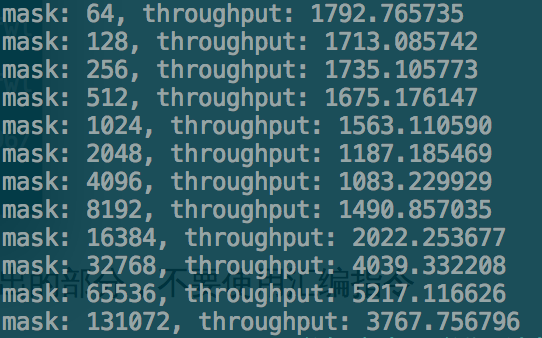
\includegraphics[width=12cm]{5.png}
        \caption{数据缓存相连度程序输出}
        \label{fig5}
      \end{figure}

      \begin{figure}[htbp]
        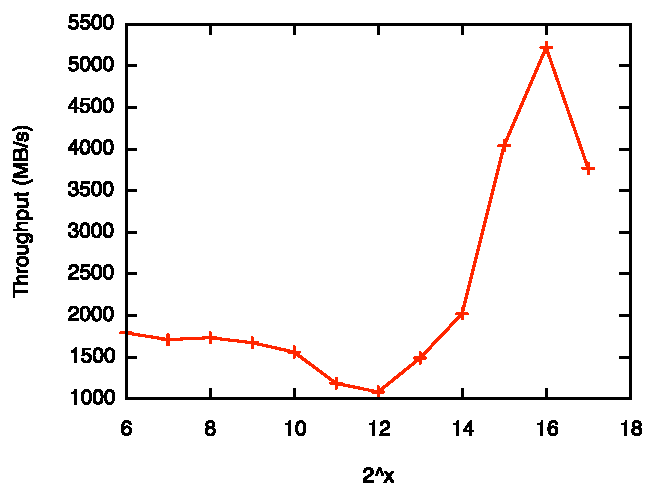
\includegraphics[width=12cm]{6.pdf}
        \caption{数据缓存相连度数据}
        \label{fig6}
      \end{figure}
      \clearpage
  \section{对所给程序\texttt{matrix\_mul.cpp}进行优化}
    对于$A\times B=C$的矩阵乘法.对于指数的顺序,一共有三种方式.其中$ijk$和$jik$等效,$jki$和$kji$等效,$kij$和$ikj$等效.

    根据\textit{Computer Systems A Programmer's Perspective}上的结论,有如表\ref{tab1}所示结论.

    所以只要采用$kij$或者$ikj$方式,就能大幅利用空间局部性提高效率.经测试使用原来的方法耗时\SI{7658105}{\ms},使用$ikj$方式只需\SI{2790251}{\ms}.

    \begin{table}[htbp]
      \centering
      \begin{tabular}{p{1.5cm} p{1.5cm} p{1.5cm} p{1.5cm} p{1.5cm} p{1.5cm} p{1.5cm}}
        Matrix multiply version & Loads per iter. & Stores per iter. & A misses per iter. & B misses per iter. & C misses per iter. & Total misses per iter. \\
        \hline
        $ijk$ \& $jik$ & 2 & 0 & 0.25 & 1.00 & 0.00 & 1.25 \\
        $jki$ \& $kji$ & 2 & 1 & 1.00 & 0.00 & 1.00 & 2.00 \\
        $kij$ \& $ikj$ & 2 & 1 & 0.00 & 0.25 & 0.25 & 0.50 \\
      \end{tabular}
      \caption{矩阵乘法效率}
      \label{tab1}
    \end{table}
    \clearpage
  \section{测量数据缓存的写回策略}
    \subsection{实验原理}
    \subsection{实验结果和数据分析}
\end{document}
